\documentclass[11pt,a4paper]{article}
\usepackage[spanish,es-nodecimaldot]{babel}	% Utilizar español
\usepackage[utf8]{inputenc}					% Caracteres UTF-8
\usepackage{graphicx}						% Imagenes
\usepackage[hidelinks]{hyperref}			% Poner enlaces sin marcarlos en rojo
\usepackage{fancyhdr}						% Modificar encabezados y pies de pagina
\usepackage{float}							% Insertar figuras
\usepackage[textwidth=390pt]{geometry}		% Anchura de la pagina
\usepackage[nottoc]{tocbibind}				% Referencias (no incluir num pagina indice en Indice)
\usepackage{enumitem}						% Permitir enumerate con distintos simbolos
\usepackage[T1]{fontenc}					% Usar textsc en sections
\usepackage{amsmath}						% Símbolos matemáticos
\usepackage{listings}
\usepackage{color}

 
\definecolor{codegreen}{rgb}{0,0.6,0}
\definecolor{codegray}{rgb}{0.5,0.5,0.5}
\definecolor{codepurple}{rgb}{0.58,0,0.82}
\definecolor{backcolour}{rgb}{0.99,0.99,0.99}
 
\lstdefinestyle{mystyle}{
    backgroundcolor=\color{backcolour},   
    commentstyle=\color{codegreen},
    keywordstyle=\color{magenta},
    numberstyle=\tiny\color{codegray},
    stringstyle=\color{codepurple},
    basicstyle=\footnotesize,
    breakatwhitespace=false,         
    breaklines=true,                 
    captionpos=b,                    
    keepspaces=true,                 
    numbers=left,                    
    numbersep=5pt,                  
    showspaces=false,                
    showstringspaces=false,
    showtabs=false,                  
    tabsize=2
}
 
\lstset{style=mystyle, language=Python}

% Comando para poner el nombre de la asignatura
\newcommand{\asignatura}{Inteligencia de Negocio}
\newcommand{\autor}{José María Sánchez Guerrero}
\newcommand{\titulo}{Práctica 2}
\newcommand{\subtitulo}{Visualización y segmentación}

% Configuracion de encabezados y pies de pagina
\pagestyle{fancy}
\lhead{\autor{}}
\rhead{\asignatura{}}
\lfoot{Grado en Ingeniería Informática}
\cfoot{}
\rfoot{\thepage}
\renewcommand{\headrulewidth}{0.4pt}		% Linea cabeza de pagina
\renewcommand{\footrulewidth}{0.4pt}		% Linea pie de pagina

\begin{document}
\pagenumbering{gobble}

% Pagina de titulo
\begin{titlepage}

\begin{minipage}{\textwidth}

\centering

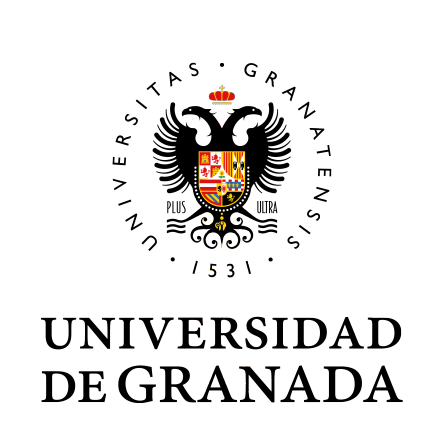
\includegraphics[scale=0.5]{img/ugr.png}\\

\textsc{\Large \asignatura{}\\[0.2cm]}
\textsc{GRADO EN INGENIERÍA INFORMÁTICA}\\[1cm]

\noindent\rule[-1ex]{\textwidth}{1pt}\\[1.5ex]
\textsc{{\Huge \titulo\\[0.5ex]}}
\textsc{{\Large \subtitulo\\}}
\noindent\rule[-1ex]{\textwidth}{2pt}\\[3.5ex]

\end{minipage}

\vspace{0.5cm}

\begin{minipage}{\textwidth}

\centering

\textbf{Autor}\\ {\autor{}}\\[2.5ex]
\textbf{Rama}\\ {Sistemas de Información}\\[2.5ex]
\vspace{0.3cm}


\includegraphics[scale=0.3]{img/etsiit.jpeg}

\vspace{0.3cm}
\textsc{Escuela Técnica Superior de Ingenierías Informática y de Telecomunicación}\\
\vspace{1cm}
\textsc{Curso 2020-2021}
\end{minipage}
\end{titlepage}

\pagenumbering{arabic}
\tableofcontents
\thispagestyle{empty}				% No usar estilo en la pagina de indice

\newpage

\setlength{\parskip}{1em}



\section{Visualización}

Partiendo del dataset de mamografías de la práctica anterior, tendremos que realizar distintas visualizaciones y analizar los
datos que tenemos para cada uno de los preprocesamientos. En mi caso, yo ya mostré en mi práctica anterior una pequeña visualización
de los datos (y que los volveré a mostra para analizarlos mejor), pero en esta completaremos más detalladamente la información.

\subsection{Visualización de las medidas}

Lo primero que pudimos observar, es que tenemos tanto datos numéricos, como datos categóricos. También vimos que hay varias celdas
con datos erróneos o perdidos (representados con el valor $NaN$):

\begin{table}[H]
    \centering
    \resizebox{325px}{!}{%
    \begin{tabular}{|c|c|c|c|c|c|c|}
    \hline
    \textbf{} & \textbf{BI-RADS} & \textbf{Age} & \textbf{Shape} & \textbf{Margin} & \textbf{Density} & \textbf{Severity} \\ \hline
    \textbf{0} & 5.0 & 67.0 & L & 5.0 & 3.0 & maligno \\ \hline
    \textbf{1} & 4.0 & 43.0 & R & 1.0 & NaN & maligno \\ \hline
    \textbf{2} & 5.0 & 58.0 & I & 5.0 & 3.0 & maligno \\ \hline
    \textbf{3} & 4.0 & 28.0 & R & 1.0 & 3.0 & benigno \\ \hline
    \textbf{4} & 5.0 & 74.0 & R & 5.0 & NaN & maligno \\ \hline
    \end{tabular}%
    }
\end{table}

Debido a esto, es importante procesarlos para que nuestros algoritmos funcionen correctamente. La técnica que elegimos en la práctica
anterior fue simplemente la de eliminar estos datos erróneos, con el siguiente resultado:

\begin{figure}[H]
    \centering
    
    \begin{minipage}{0.5\textwidth}
        \centering
        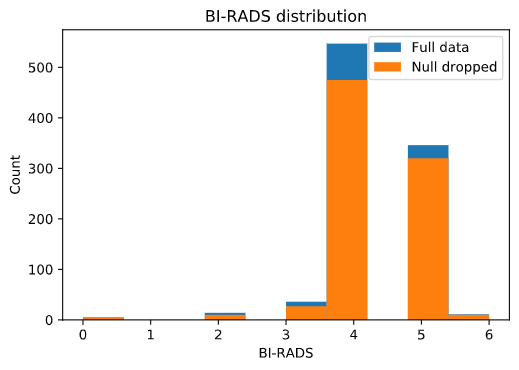
\includegraphics[scale=0.35]{img/birads-distribution.png}
    \end{minipage}%
    \begin{minipage}{0.5\textwidth}
        \centering
        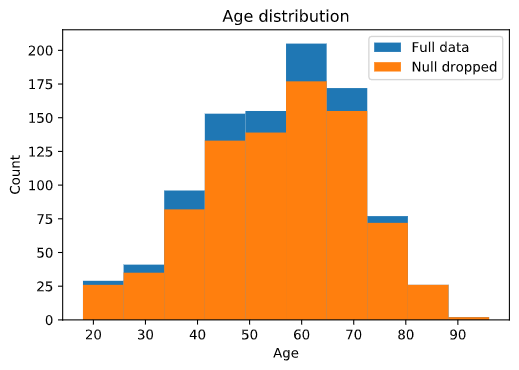
\includegraphics[scale=0.35]{img/age-distribution.png}
    \end{minipage}
    
\end{figure}
    
    
\begin{figure}[H]
    \centering
    
    \begin{minipage}{0.5\textwidth}
        \centering
        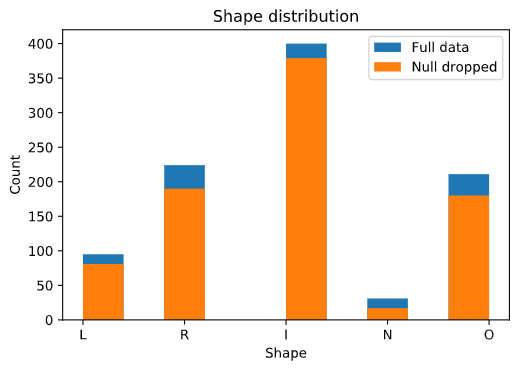
\includegraphics[scale=0.35]{img/shape-distribution.png}
    \end{minipage}%
    \begin{minipage}{0.5\textwidth}
        \centering
        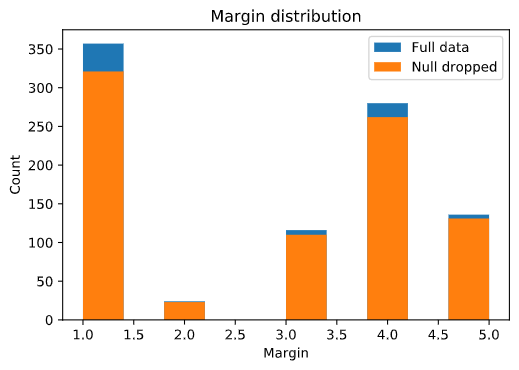
\includegraphics[scale=0.35]{img/margin-distribution.png}
    \end{minipage}
    
\end{figure}
    
    
\begin{figure}[H]
    \centering
    
    \begin{minipage}{0.5\textwidth}
        \centering
        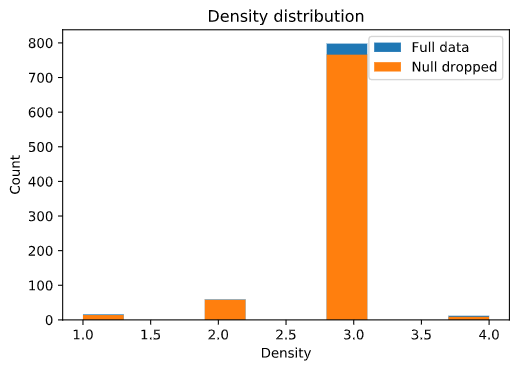
\includegraphics[scale=0.35]{img/density-distribution.png}
    \end{minipage}%
    \begin{minipage}{0.5\textwidth}
        \centering
        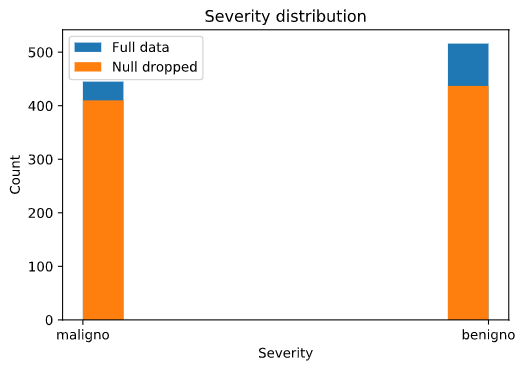
\includegraphics[scale=0.35]{img/severity-distribution.png}
    \end{minipage}
    
\end{figure}
    
Otra estrategia de preprocesamiento que podríamos haber utilizado es la de completar esos valores con datos. Esto a veces puede
no tener sentido, ya que en algunos atributos, como por ejemplo la edad, no vas a asignarle a todos los datos que faltan el valor
de 0 años. Para estos casos veremos otra solución más adelante.

Sin embargo, tenemos atributos como la forma (''\textit{Shape}''), que ya de por sí tienen un valor ''No definido'' con varios
datos en él. Gracias a esto, los datos erróneos o nulos del dataset los podemos meter en esta categoría. 
\begin{figure}[H]
    \centering
    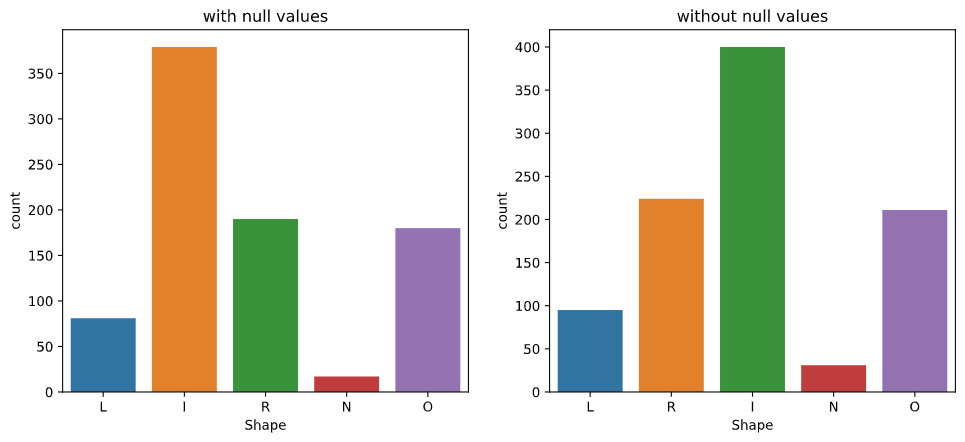
\includegraphics[scale=0.35]{img/shape-refill.png}
\end{figure}

\newpage

¿Qué estrategia diferente podemos utilizar entonces para el resto sin eliminarlos ni poner valores sin sentido? Tenemos varias
opciones. La primera que se nos viene a la cabeza es hacer la media la media entre todos los parámetros y devolver su resultado,
pero esto puede \textit{boostear} mucho un valor y darle demasiada importancia. Es una buena medida en caso de que haya pocos
datos erróneos o nulos, ya que no va a a desbalancearlo mucho.

Sin embargo, nosotros vamos a utilizar interpolación con el método '\textit{nearest}' para que tenga en cuenta los valores de los
índices más cercanos y así distribuir un poco más los nuevos valores. Los resultados que hemos obtenido para el parámetro edad
han sido los siguientes:
\begin{figure}[H]
    \centering
    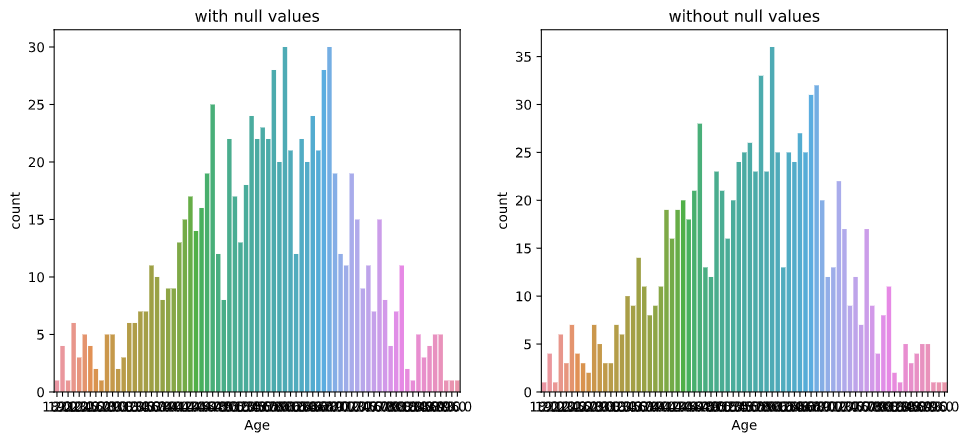
\includegraphics[scale=0.35]{img/age-refill.png}
\end{figure}

Hay que fijarse bien ya que son muchos los valores que puede adoptar la edad, pero vemos cómo no hay ningún valor muy por encima de
lo normal ni que hayan sido \textit{boosteados} en exceso. Con otros valores, como la densidad, también lo podemos hacer, pero
se aprecia un poco menos la diferencia porque hay menos variedad de datos y el 3 destaca sobre todos los demás.
\begin{figure}[H]
    \centering
    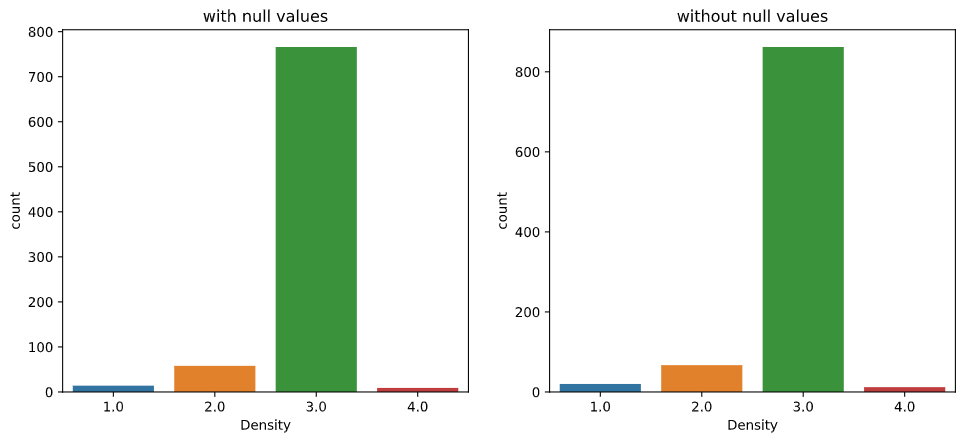
\includegraphics[scale=0.35]{img/density-refill.png}
\end{figure}

Por último, vamos a hacer una media en los atributos que faltan para poder ver también cómo trabaja esta manera de preprocesado.
Podremos observar cómo algunos datos apenas cambian, o es difícil apreciarlo; pero otros, como por ejemplo el valor 3 en 'Margin'
sube bastante, llegando al punto de superar el valor 5 y dándole más importancia en el dataset. No quiere decir que esté mal, ya
que no se sabe cómo serían esos datos en realidad o si pueden venir más datos como estos en un futuro. Pero hay que tener cuidado
porque son datos 'inventados' y, en este caso, originalmente el dataset le da más importancia al 5 que al 3, y lo estamos cambiando.

\begin{figure}[H]
    \centering
    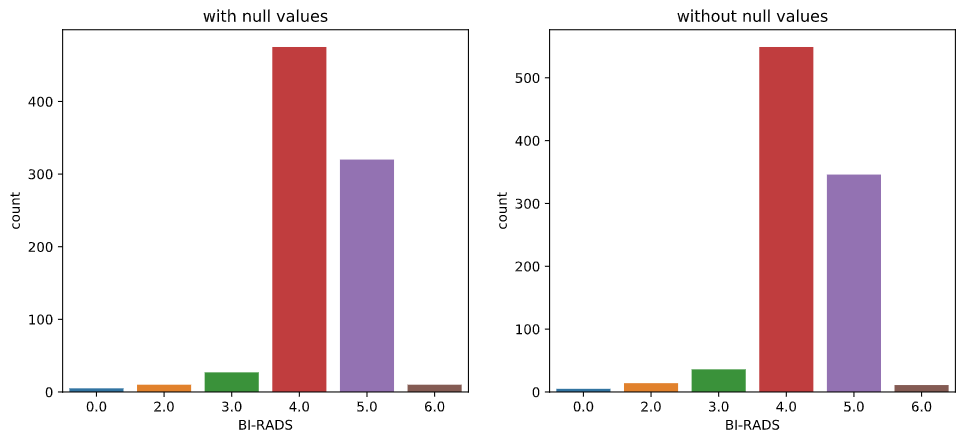
\includegraphics[scale=0.35]{img/birads-refill.png}
\end{figure}

\begin{figure}[H]
    \centering
    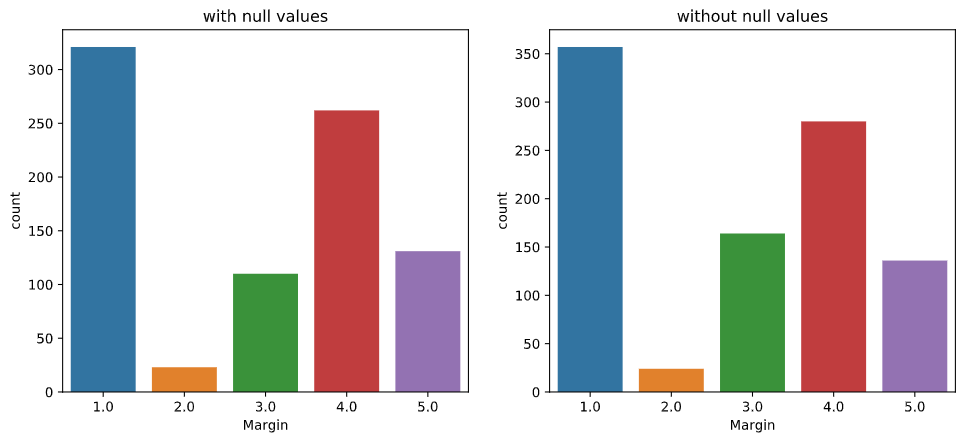
\includegraphics[scale=0.35]{img/margin-refill.png}
\end{figure}


\newpage
\subsection{Gráficas de curva ROC}
No vamos a comentar de nuevo el código, la declaración de los algoritmos, ni la explicación de cómo funcionan, ya que lo hicimos
en la práctica anterior. Únicamente decir que se ha utilizado también un '\textit{Label Encoder}', para los atributos que no son
numéricos, y que se ha hecho la misma división de los datos.

La diferencia con la práctica es que vamos a utilizar simplemente el método \textit{fit()} para entrenar los datos, y después,
con el conjunto de test, hacemos todas las curvas ROC y las mostramos en una sóla gráfica. Este ha sido el resultado:

\begin{figure}[H]
    \centering
    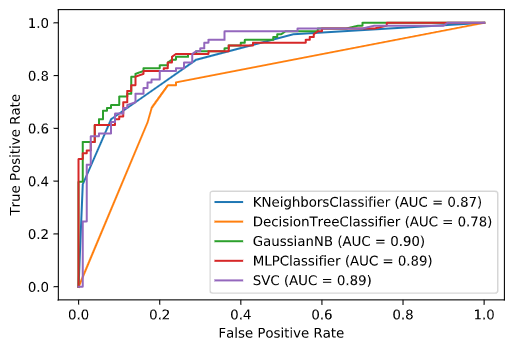
\includegraphics[scale=0.5]{img/curva-roc.png}
\end{figure}

Esta curva representa dos parámetros: tasa de verdaderos positivos y tasa de falsos positivos. El área que hay debajo de la curva
(cálculo de la integral) nos dice cómo es el rendimiento del modelo. Es decir, una curva perfecta subiría hasta la coordenada
$(0,1)$, y su integral daría como resultado 1 (100\% de tasa de verdaderos positivos).


\subsection{Análisis de atributos}
En esta sección realizaremos una serie de representaciones de los distintos atributos para así intentar encontrar alguna relación
entre ellos. Algunos tipos de gráficos ya los hemos utilizado, como puede ser el \textit{countplot}, y el cual lo podemos utilizar
simplemente para saber la cantidad de datos que hay, o la cantidad de benignos y malignos que tenemos:

\begin{figure}[H]
    \centering
    
\includegraphics[scale=0.5]{img/severity-count.png}
\end{figure}

Este gráfico no nos sirve más allá que para contar el número de datos que tiene cada clase, por lo que ya no nos va a servir de
mucho tras haber hecho todo lo anterior. Además de que este tipo de gráfico tampoco nos es útil para relacionar 2 o más categorías.

A continuación, vamos a ver uno llamado \textit{scatterplot}, el cual es un diagrama de dispersión que muestra los datos en forma
de puntos. La posición de cada uno de los puntos viene determinada por un atributo para cada uno de los ejes. Con el diagrama de
dispersión así se podría extraer algún tipo de relación entre los dos atributos, pero para lo que realmente es útil es este tipo
de gráficos en $Seaborn$, es por su capacidad de categorizar los puntos con el atributo objetivo, en nuestro caso la severidad.
Vamos a ver la relación que existe entre la edad y el margen de masa:

\begin{figure}[H]
    \centering
    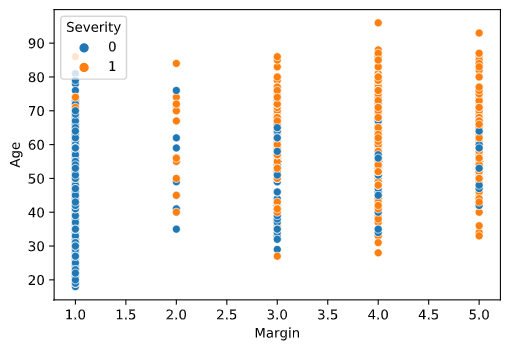
\includegraphics[scale=0.5]{img/scatter-age-margin.png}
\end{figure}

Podemos ver que la relación entre la edad y el margen es prácticamente inexistente, ya que los datos están distribuidos más o menos
de forma equilibrada. No obstante, en cuanto a la severidad, si que podemos ver una clara tendencia a ir hacia la izquierda los
benignos y a la derecha los malignos. Esto quiere decir que cuanto menor sea el margen de masa, más posibilidades hay de que sea
benigno, y viceversa. En cuanto a la edad, lo que vemos no nos dice mucho, ya que hay benignos y malignos repartidos por todas las
edades (es cierto que a edades más bajas vemos un poco más de color azul y a edades más altas naranja, pero nada relevante o para
poder sacar conclusiones).

En la siguiente gráfica, una \textit{boxplot}, vamos a poder observar mejor mejor la diferencia que hemos comentado anteriormente,
porque es un tipo de gráfica (llamada también diagrama de caja) que representa, tanto los cuartiles de los datos con la caja, como
el resto de la distribución con los 'bigotes' que salen de ella.

\begin{figure}[H]
    \centering
    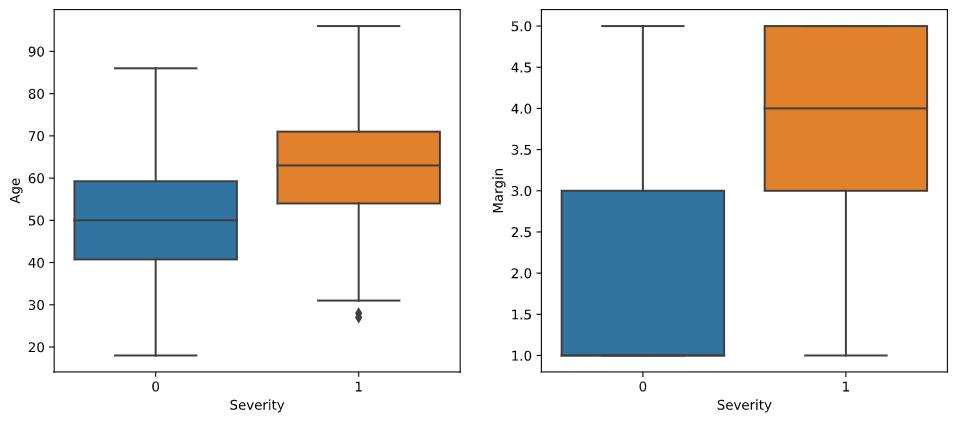
\includegraphics[scale=0.4]{img/boxplot-age-margin.png}
\end{figure}

Ahora vemos más claramente lo que comentábamos anteriormente, y es que la edad apenas es relevante en cuanto a la severidad, ya que
las dos cajas están más o menos en mitad del gráfico, con un pequeña tendencia del naranja a ser más severo. Sin embargo, el margen
de masa si podemos ver cómo hay una marcada diferencia entre las dos cajas, por lo que deducimos que este valor si es más importante
a la hora de decidir la severidad del dato.

Otro punto bueno de este tipo de diagrama es que no tiene en cuenta los valores atípicos para el cálculo de estos parámetros mediante
una función que es un función del rango intercuartil.

\newpage
Hacer estas gráficas para todos los atributos del dataset puede resultar bastante engorroso, sobre todo si tenemos una gran cantidad
de atributos. Los gráficos tipo \textit{pairplot} es la mejor solución para este problema. Estos crean un grid con todas las variables
numéricas de nuestro dataset y comparan unas con otras, al igual que acabamos de hacer con los diagramas de dispersión y cajas vistos.
Las gráficas de la diagonal se tratan se forma diferente: muestran la distribución marginal de los datos en cada columna (por decirlo
de otra forma, la probabilidad de que un dato adopte un determinado valor u otro).

Dicho esto, vamos a ver cómo se vería un \textit{pairplot} de nuestro dataset:

\begin{figure}[H]
    \centering
    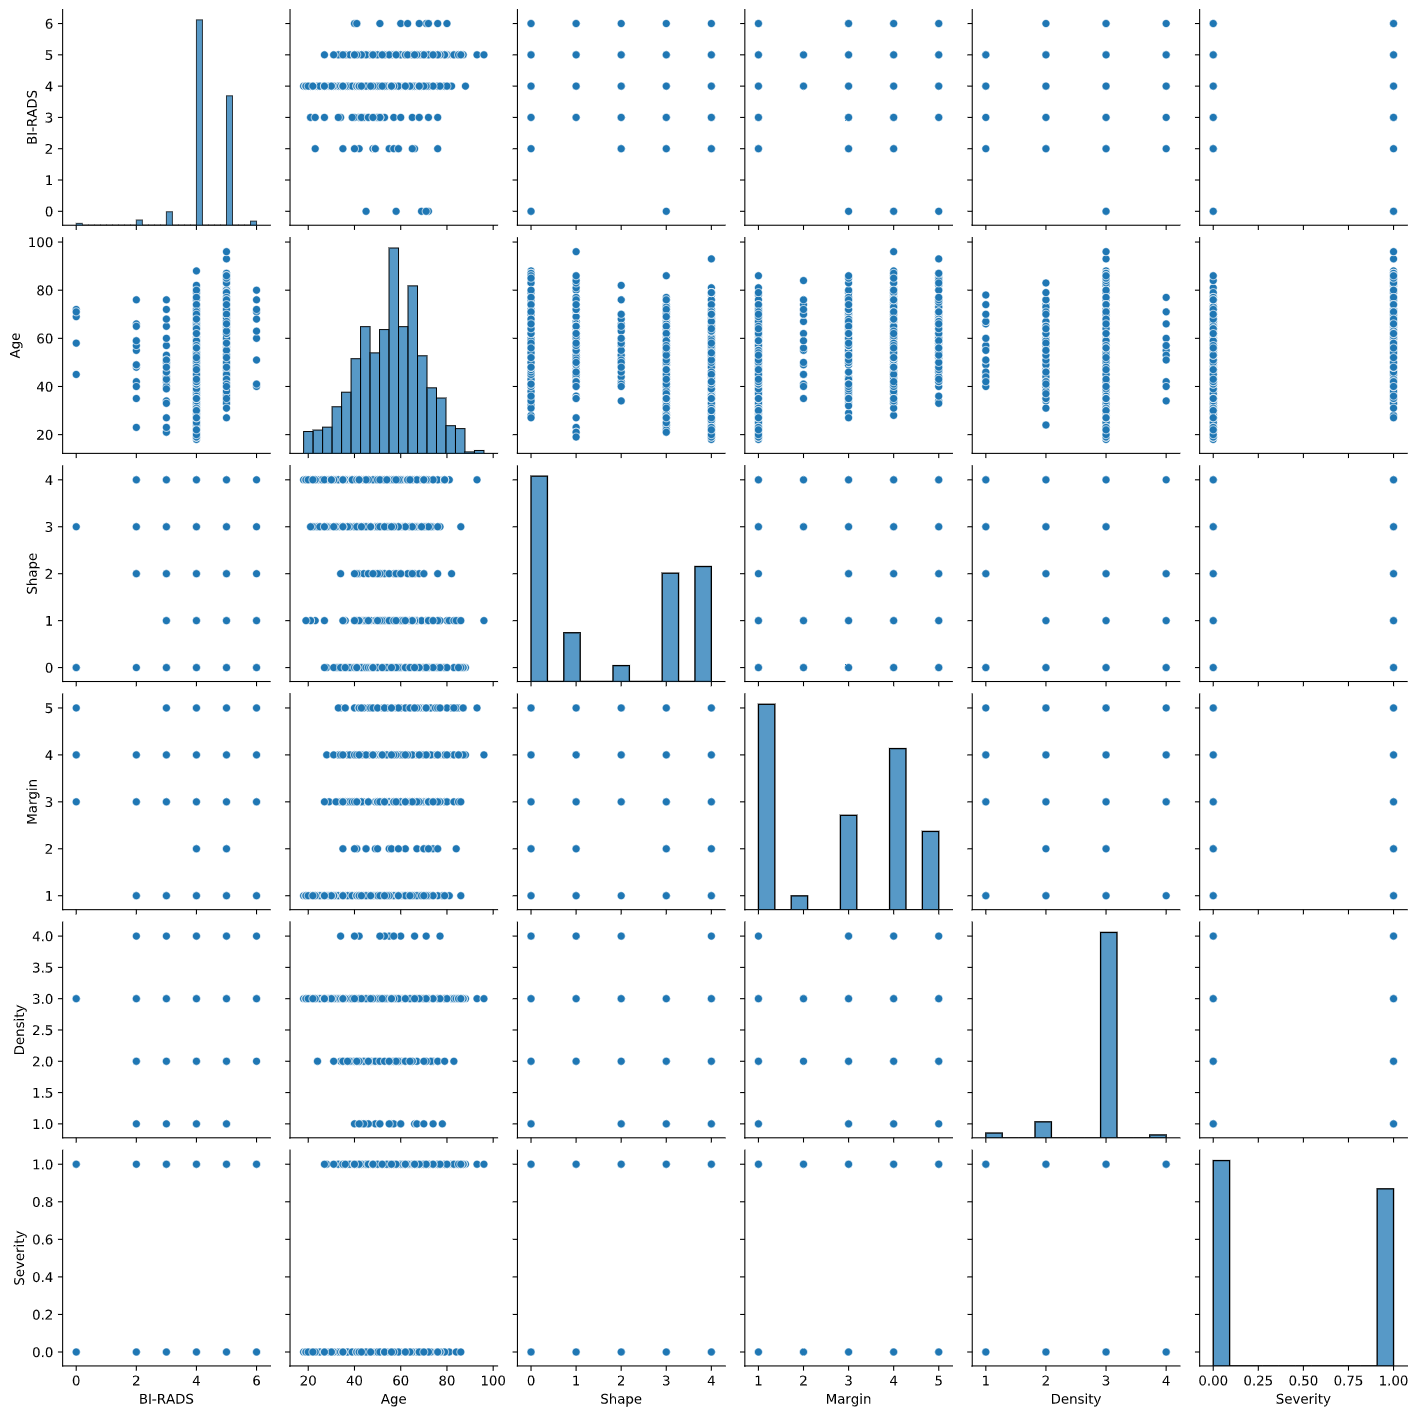
\includegraphics[scale=0.25]{img/pairplot.png}
\end{figure}

Podemos observar los gráficos de dispersión para cada una de las variables y ver cómo están repartidos los datos, al igual que la
distribución de los valores para cada atributos. Pese a esto, nos falta algo imprescindible, y es que la severidad está como otro
atributo normal en vez de ser nuestro atributo objetivo.

Para ello, utilizaremos el parámetro ''\textit{hue='Severity'} '' con el que mapearemos la gráfica en función del atributo pasado como
parámetro:

\begin{figure}[H]
    \centering
    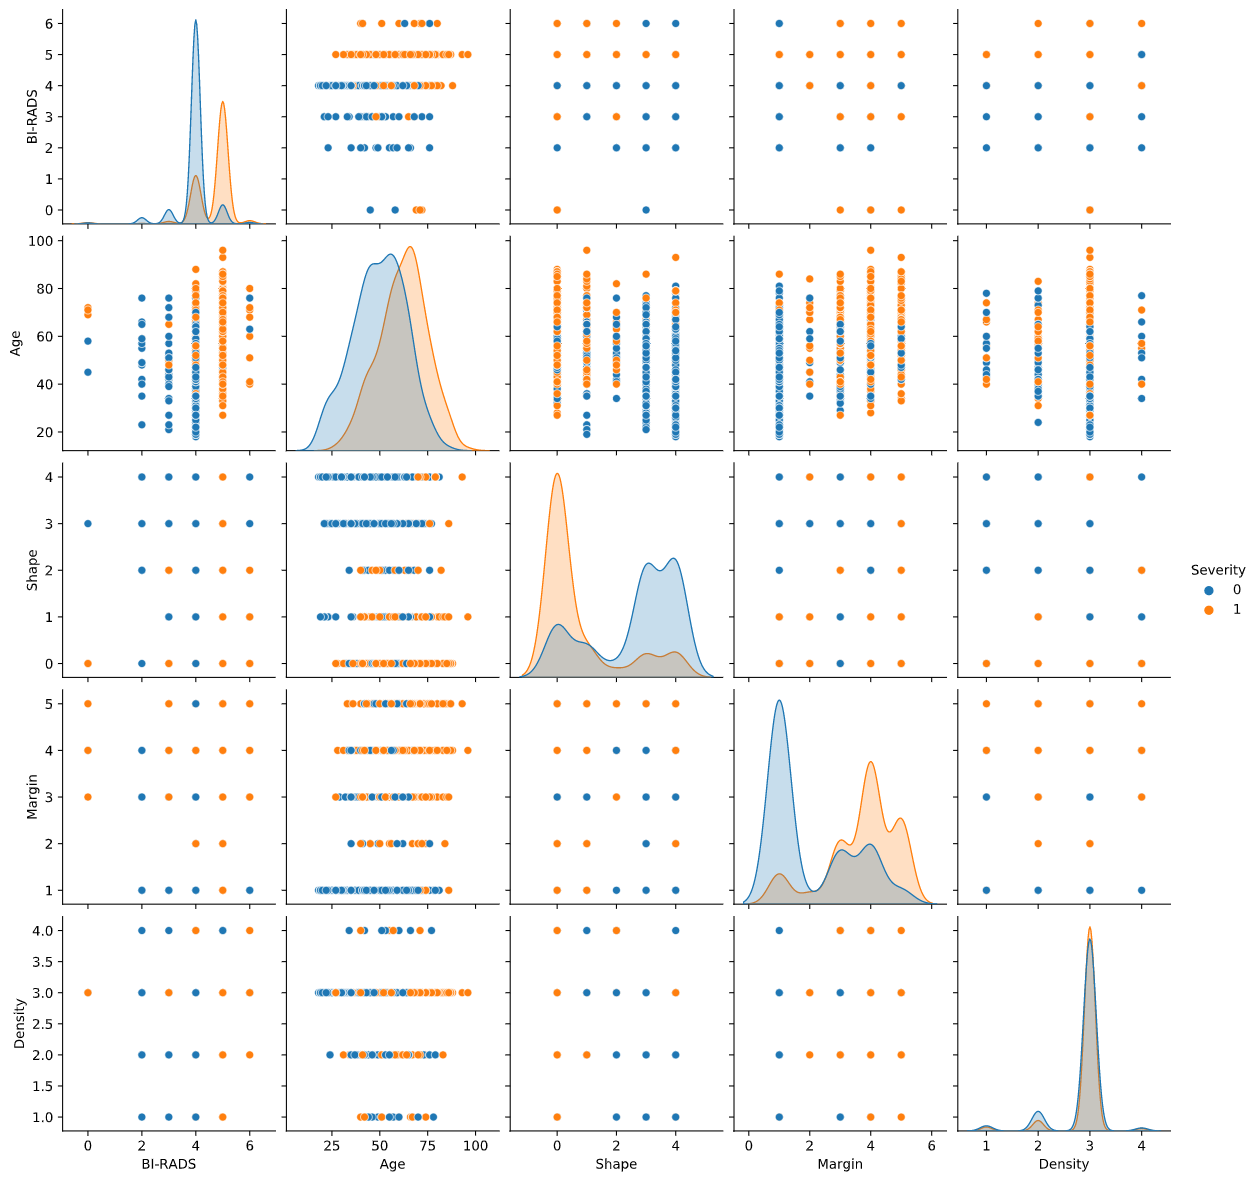
\includegraphics[scale=0.3]{img/pairplot-hue.png}
\end{figure}

Aquí sí que podemos diferenciar claramente los tumores benignos y malignos para cada uno de los atributos. Por ejemplo, podemos ver
lo que dijimos anteriormente del parámetro edad y cómo está ligeramente diferenciado pero sin ser excesivamente relevante. También
observamos que la densidad por ejemplo, es un dato prácticamente irrelevante para determinar la severidad del tumor, ya que podríamos
decir que están totalmente superpuestos ambos colores. Si ahora nos fijamos en el gráfico de dispersión entre la edad y la densidad,
se puede ver claramente cómo hay puntos de todos los colores distribuidos por todo el espacio de coordenadas, y que apenas se puede
diferenciar ningún patrón.

Por otra parte, si que podemos sacar datos relevantes. Por ejemplo, tanto la forma como el margen de masa tienen dos zonas bastante
bien diferenciadas. Es decir, si el margen de masa tiene un valor de 1, hay una gran probabilidad de que el tumor sea benigno, en
caso contrario, es más probable que sea maligno, pero con un porcentaje de acierto más bajo, ya que tenemos también bastantes casos de
tumor benigno con estos valores.

Analizando todos los demás, podemos sacar más conclusiones bastante interesantes, como puede ser la del valor 5 de BI-RADS. Si nos
fijamos en la distribución, ya podemos ver un pico naranja importante sin apenas casos azules en él; pero si vamos observando cada
uno de los gráficos de dispersión para el resto de atributos, vemos que para \textit{BI-RADS = 5} únicamente hay un solo caso benigno,
mientras que el resto son malignos. Al contrario nos pasa con el valor 2 de BI-RADS, y es que no encontramos ningún caso de tumor
maligno con él.

Al igual que este caso que comentamos, podemos encontrar más por todas las gráficas. También podremos ver relaciones entre atributos,
como la de densidad-margen, en la cuál vemos más naranja cuanto más a la derecha (o arriba, dependiendo de la que estemos mirando) de
la nube de puntos vayamos.




\section{Segmentación}

\subsection{Introducción}
En este apartado, vamos a estudiar un conjunto de datos publicados por la Dirección General de Tráfico (DGT) sobre los accidentes de
tráfico en España entre los años 2008 y 2015. Se pretende comprender mejor cómo suceden los accidentes, es decir, encontrar variables
que caractericen los accidentes, grupos de accidentes similares y en general los factores comunes que solemos encontrar en ellos, con
la intención de detectar el problema y, presumiblemente, intentar hacer algo al respecto.

El dataset proporcionado en la web de la asignatura, que será sobre el que trabajemos, ya está procesado a partir de la fuente original.
Cuenta con 89.519 datos o accidentes, y cada uno de ellos tiene 32 atributos distintos sobre el mes, la hora, total de víctimas, total
de muertos, heridos, tipo de vía, luminosidad, visibilidad, etc\dots

A continuación, vamos a comentar los dos algoritmos de agrupamiento utilizados para cada caso de estudio. Uno de ellos, como se nos
dice en el enunciado, es el K-Means, y el otro que he elegido ha sido el DBSCAN:
\begin{itemize}
    \item \textbf{K-Means}. Este algoritmo agrupa los datos en $k$ grupos distintos, dependiendo del valor que le demos. Funciona de
          la siguiente manera: se parten de $k$ centros iniciales y, para cada uno de los datos, se le asigna un \textit{cluster}
          perteneciente al centro más cercano. Posteriormente, se recalcula el centro y se pasa al siguiente dato. Este algoritmo es
          relativamente eficiente y suele terminar en un óptimo local. Por otro lado, es un algoritmo sensible al ruido y sólo es
          indicado para \textit{clusters} convexos.
    \item \textbf{DBSCAN}. Este un algoritmo basado en densidad que no utiliza centroides, sino que utiliza dos parámetros para definir
          la densidad: $eps$, que nos dice cuando un objeto es alcanzable por otro; y $min\_samples$, que es el número mínimo de datos
          por los que podemos alcanzar otro. Veámoslo mejor con la siguiente imagen:
          \begin{figure}[H]
            \centering
            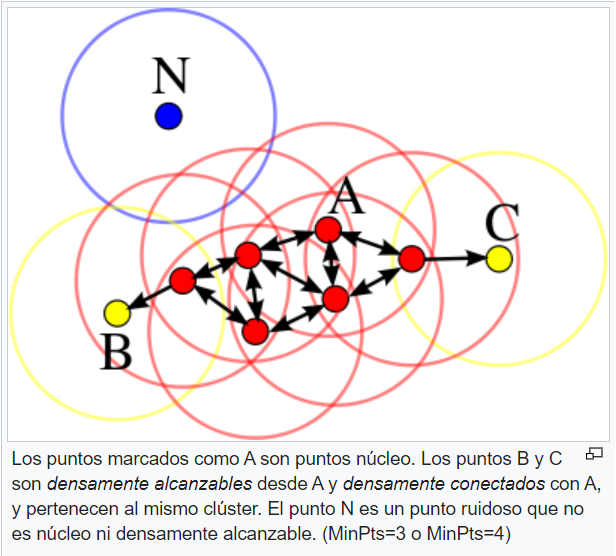
\includegraphics[scale=0.45]{img/dbscan.png}
            \caption{https://es.wikipedia.org/wiki/DBSCAN}
        \end{figure}
        Los grupos que estén etiquetados como -1 representarán los datos con ruido, que no pueden ser agrupados.
\end{itemize}

Ahora vamos a analizar las métricas de rendimiento que vamos a utilizar para comparar los resultados:

\begin{itemize}
    \item \textbf{Silhouette}. Te dice cómo de similares son los objetos de un cluster comparado con los otros clusters distintos.
          Se guía por un rango de valores, donde el -1 significa que el agrupamiento no está bien hecho, 1 significa que los datos
          están concentrados y separados del resto de clusters, y 0 que los clusters están uno encima de otro.
    \item \textbf{Calinski-Harabaz}. Es la razón entre la dispersión intra-clusters y la dispersión inter-clusters. Cuanto más alto
          sea el valor, más densos y mejor separados están unos clusters de otros.
    \item \textbf{Número de clústers}. No es tanto una métrica de rendimiento, pero la cantidad de clusters que pongamos nos puede
          determinar por completo lo que obtengamos en todo lo demás. Es decir, tendremos que ajustarlo para ver qué número es el
          que mejor se adapta a nuestro modelo.
\end{itemize}

Nuestros casos de estudio se van a centrar en obtener información sobre los accidentes entre 2 comunidades autónomas distintas. Lo
que queremos es ver si hay alguna diferencia entre ellas y buscar algún factor relevante que pueda causar esta diferencia, como por
ejemplo el clima, la hora a la que se producen, tipos de calzadas, o si simplemente unos conducen mejor y otros peor.


\subsection{Caso de estudio 1. Andalucía}

Las variables que vamos a utilizar en este caso van a ser las siguientes:

\begin{itemize}
    \item \textbf{HORA}. Un número entre 0 y 24 que representa la hora a la que se ha producido. En ocasiones tenemos datos decimales
          que representan los minutos (por ejemplo, 19.50 representa las siete y media de la tarde).
    
    \item \textbf{DIASEMANA}. Representa el día de la semana en el que ha sucedido el accidente.
    
    \item \textbf{TIPO\_VIA}. Indica la vía donde se ha producido el accidente. Tras realizar '\textit{labelEncoder}' para asignar un
          valor numérico a cada una de las etiquetas, este ha sido el resultado:

          'Autopista': 0 \quad 'Autovía': 1,\quad 'Camino vecinal': 2,\quad 'Otro tipo': 3,\quad 'Ramal de enlace': 4, \quad
          'Vía convencional': 5,\quad 'Vía convencional con carril lento': 6,\quad 'Vía de servicio': 7,\quad 'Vía para automóviles': 8
    
    \item \textbf{LUMINOSIDAD}. Es la cantidad de luz que había en la zona del accidente. Al igual que antes, hemos hecho la codificación
          numérica, con el siguiente resultado:
    
          'Crepúsculo': 0, 'Noche: iluminación insuficiente': 1, 'Noche: iluminación suficiente': 2, 'Noche: sin iluminación': 3,
          'Pleno día': 4
    
    \item \textbf{FACTORES\_ATMOSFERICOS}. Indica la cómo estaba la meteorología en el momento del accidente. La codificación nos ha
          devuelto el siguiente resultado:

          'Buen tiempo': 0, 'Granizando': 1, 'Lloviznando': 2, 'Lluvia fuerte': 3, 'Nevando': 4, 'Niebla intensa': 5, 'Niebla ligera': 6,
          'Otro': 7, 'Viento fuerte': 8
\end{itemize}

Una vez analizados los parámetros, vamos a pasar a crear nuestro algoritmo de clustering. El primero de ellos va a ser el ya comentado
\textit{KMeans}. Su parámetro más importante es el $k$, y sin conocer un problema detalladamente, como es nuestro caso, es difícil
seleccionar un número de clusters inicial. Por esto, vamos a realizar un pequeño estudio sobre qué valor escoger.

Realizamos varias ejecuciones con valores entre 2 y 10, y ejecutamos el algoritmo. Para saber cuál de ellas ha ido mejor, nos vamos
a guiar por las métricas de rendimiento comentadas anteriormente. Este ha sido el resultado:

% Please add the following required packages to your document preamble:
% \usepackage{graphicx}
\begin{table}[H]
    \centering
    \begin{tabular}{|c|c|c|}
    \hline
    \textbf{Clusters} & \textbf{Silhouette} & \textbf{Calinsky} \\ \hline
    2 & 0.284494 & 5530.132494 \\ \hline
    3 & 0.325936 & 6023.345251 \\ \hline
    4 & 0.353282 & 5605.199947 \\ \hline
    5 & 0.341677 & 5039.045342 \\ \hline
    6 & 0.247302 & 4744.881579 \\ \hline
    7 & 0.260930 & 4505.936416 \\ \hline
    8 & 0.255387 & 4245.012708 \\ \hline
    9 & 0.262860 & 3992.702383 \\ \hline
    10 & 0.283835 & 4048.522720 \\ \hline
    \end{tabular}
\end{table}

Podemos observar, que a medida que se van aumentando el número de clusters, los coeficientes van disminuyendo. Sobre todo, esto
afecta más al coeficiente Calinsky, debido a que las diferencias entre uno y otro son menores (pese a estar más concentrados). El
coeficiente Silhouette vemos que a partir de los 5 clusters da un bajón notable, por lo que un agrupamiento tan disperso hace más
complicado la diferenciación de los elementos frontera.

Finalmente, vamos a elegir 4 clústers distintos para continuar con el problema. Es cierto que 3 clusteres tienen mayor coeficiente
Calinsky, no obstante, pienso que la diferencia entre este y los demás no es tan notable como la del coeficiente Silhouette.

\begin{figure}[H]
    \centering
    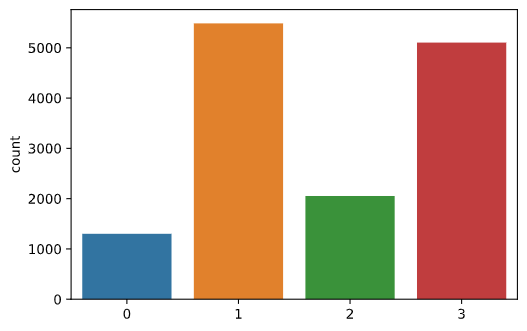
\includegraphics[scale=0.4]{img/cluster-distribution-and.png}
\end{figure}

Esta es la distribución de cada uno de los grupos generados por la cantidad de elementos que hay en cada uno de ellos. Podemos ver
que los que más han destacado han sido el 1 y el 3. Para analizar estos grupos detalladamente, vamos a visualizar tanto los centroides
como el grid con las distintas gráfica de dispersión y distribución de los datos. Empezamos con los centroides:

\begin{figure}[H]
    \centering
    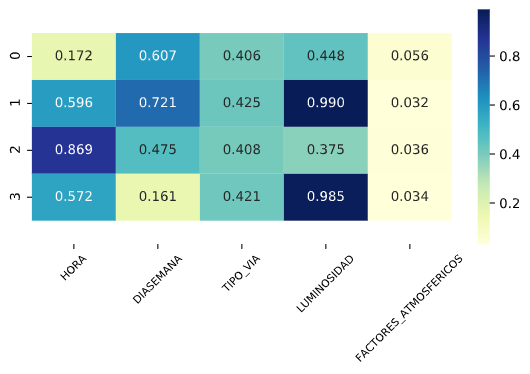
\includegraphics[scale=0.5]{img/centroides-and.png}
\end{figure}

Aquí podemos ver datos muy interesantes y que nos van a servir para poder distinguir unos grupos de otros. Por ejemplo, en cuanto
a la hora, tenemos un grupo en el cual tenemos unos valores muy altos (horas entre la tarde-noche), otros dos grupos que tienen
un valor medio (horas que transcurren durante el resto del dia), y un último grupo con unos valores más bajos (presumiblemente serán
por la madrugada). Si nos fijamos en la gráfica anterior, que muestra los elementos de cada grupo, el 1 y el 3 son los que más
datos tienen, por lo que ya podemos extraer que la mayor cantidad de accidentes se producen durante el día.

También podemos ver otros valores destacados en esta tabla, como pueden ser los de luminosidad. Un valor tan alto no quiere decir
que en el grupo 1 y 3, la mayor parte de los accidentes han sido bajo plena luz del día (como habíamos señalado tras hacer la
codificación numérica). Esto también nos cuadra con lo anterior, ya que los grupos 1 y 3 representan a los accidentes que suceden
durante el día y no por la noche o de madrugada.

Todo esto nos lleva a pensar que los grupos 1 y 3 son bastante similares y que quizás deberían estar juntos. También nos gustaría
analizar el resto de parámetros, como el día de la semana, el tipo de vía o los factores atmosféricos; así que para facilitarnos
todo este análisis, vamos a mostrar el grid con las gráficas de dispersión (\textit{pairplot}):

\begin{figure}[H]
    \centering
    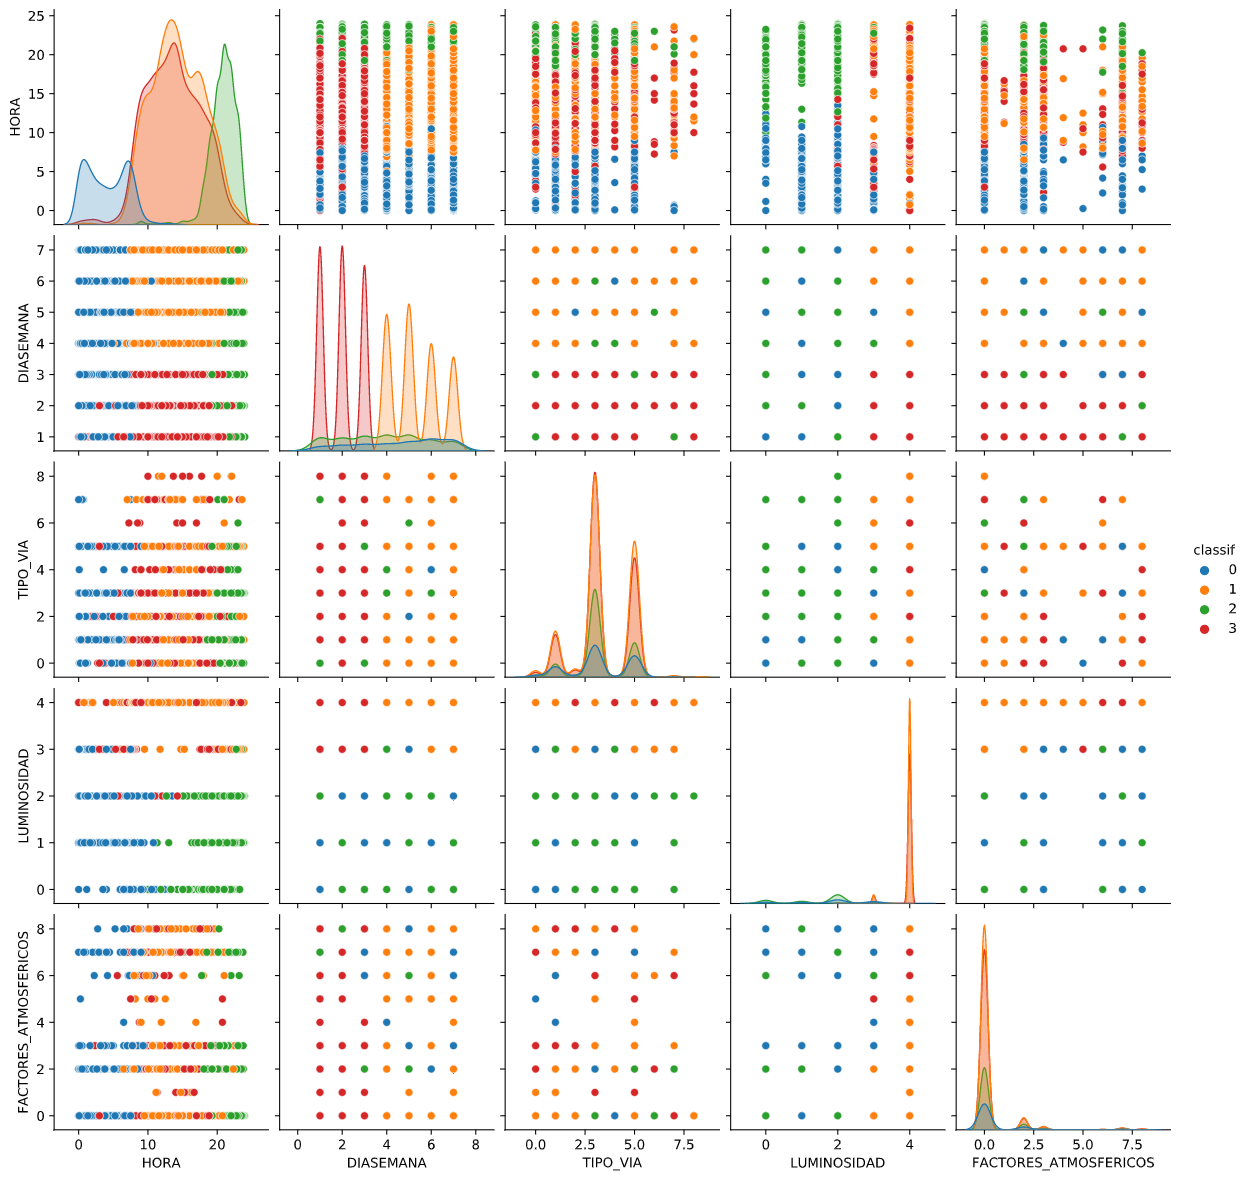
\includegraphics[scale=0.3]{img/pairplot-and.png}
\end{figure}

Vemos que gracias a este grid, somos capaces de responder a las dudas que teníamos. Empezando por los grupos 1 y 3, vemos que la
diferencia que hay entre ellos, simplemente es el día de la semana. El grupo 1 vemos que engloba los accidentes del lunes, martes
y miércoles; mientras que el grupo 3 a los del resto de días. Este dato es muy interesante, ya que uno suele pensar (en mi caso al
menos) que se producen más accidentes los fines de semana, ya sea por dar una vuelta fuera de casa, operaciones salida, etc.; sin
embargo, la cantidad de accidentes está bastante repartida por toda la semana. Los otros dos grupos también están distribuidos por
todos los días, por lo que su diferenciación con el resto se tiene que deber a otro factor, veámos cual.

Como ya habíamos adelantado analizando los centroides, el factor que diferencia a los grupos 0 y 2 son las horas del día. Podemos
observar que el grupo 1 abarca las horas de la madrugada (entre las 00:00 y las 07:00 aproximadadmente), y el grupo 2 los valores
más altos (entre las 21:00 y las 23:59 horas aproximadamente).

Pasamos ahora al tipo de vía, en el cual no hay mucho que decir. Se puede ver cómo no ha sido el factor más importante a la hora
de dividir los datos, ya que tenemos prácticamente todos los datos distribuidos por todos los valores. En las gráficas de dispersión,
evidentemente destacan los colores naranjas y rojos, pero esto se debe a que hay una mayor cantidad de datos. Por comentar algo más,
podemos observar que la mayoría de accidentes se reparten entre autovía, vía convencional y otro tipo.

Por otra parte, la luminosidad hemos obtenido más o menos lo que se esperaba. La mayoría de casos se dan en el valor 4 o 'Pleno
día', sin embargo, los grupos 0 y 2 (accidentes por la noche) se reparten por el resto de los valores. Esto en la gráfica de
distribución no lo podemos apreciar del todo bien por la cantidad de valores, pero en los gráficos de dispersión vemos cómo los
datos están claramente separados unos de otros.

Finalmente, tenemos los valores atmosféricos, en los que una gran mayoría pertenecen al valor 0 o 'Buen tiempo'. Sinceramente, me
esperaba este resultado, ya que estamos analizando los accidentes de Andalucía donde, a priori, no llueve tanto como en el otro
conjunto de datos que nos queda por analizar y que espero que nos de más juego.


\subsubsection*{DBSCAN}

Para este algoritmo comenzamos con un análisis de parámetros, al igual que hicimos con el valor $k$ en el anterior. Se busca
encontrar un valor del radio que se adapte bien a nuestro problema, junto a un mínimo de muestras para alcanzar desde un cluster
a otro. Estos han sido los resultados de la ejecución:

% Please add the following required packages to your document preamble:
% \usepackage{graphicx}
\begin{table}[H]
    \centering
    \begin{tabular}{|c|c|c|c|}
    \hline
    \textbf{epsilon} & \textbf{min\_samples} & \textbf{silhouette} & \textbf{calinsky} \\ \hline
    0.2 & 15 & 0.04407 & 490.426 \\ \hline
    0.3 & 15 & 0.43005 & 238.501 \\ \hline
    0.4 & 15 & 0.46731 & 114.703 \\ \hline
    0.2 & 20 & 0.10385 & 537.105 \\ \hline
    0.3 & 20 & 0.42490 & 245.896 \\ \hline
    0.4 & 20 & 0.46358 & 123.923 \\ \hline
    0.2 & 25 & 0.08275 & 568.401 \\ \hline
    0.3 & 25 & 0.35979 & 320.201 \\ \hline
    0.4 & 25 & 0.44782 & 165.339 \\ \hline
    \end{tabular}
\end{table}

Podemos observar que para un epsilon de 0.2 obtiene unos valores muy cercanos al 0, prácticamente negativos, por lo que podemos
descartarlo. Por lo demás, sigue una dinámica muy parecida, porque a medida que crece el coeficiente Silhouette, disminuye el
coeficiente Calinsky. Esto sucede porque DBSCAN agrupa los objetos que no pertenecen a ningún grupo, es decir, todos los datos
con ruido que obtenemos forman un cluster aparte.

En definitiva, yo me quedaría con un $eps=0.3$ y un $min\_samples=20$, ya que es un valor que iguala los dos coeficiente; sin
embargo, podemos concluir (comparando estos resultados con los del K-Means) que este algoritmo no se ajusta adecuadamente a nuestro
problema, por lo que no lo escogería.



\subsection{Caso de estudio 2. Galicia}

Para este dataset vamos a proceder de la misma forma que con el anterior, aunque en este caso no vamos a volver a explicar de nuevo
las variables a utilizar, puesto que son las mismas.

Para crear nuestro algoritmo de clustering vamos a analizar de nuevo el parámetro $k$, por si hay algún cambio. Realizamos varias
ejecuciones con valores entre 2 y 10, y ejecutamos el algoritmo. Este ha sido el resultado:

% Please add the following required packages to your document preamble:
% \usepackage{graphicx}
\begin{table}[H]
    \centering
    \begin{tabular}{|c|c|c|}
    \hline
    \textbf{Clusters} & \textbf{Silhouette} & \textbf{Calinsky} \\ \hline
    2 & 0.260078 & 1313.627673 \\ \hline
    3 & 0.280594 & 1368.089351 \\ \hline
    4 & 0.302228 & 1238.453937 \\ \hline
    5 & 0.287155 & 1143.273081 \\ \hline
    6 & 0.302304 & 1082.532618 \\ \hline
    7 & 0.303291 & 1066.656547 \\ \hline
    8 & 0.279829 & 1052.982888 \\ \hline
    9 & 0.263503 & 1025.977641 \\ \hline
    10 & 0.272481 & 1018.666117 \\ \hline
    \end{tabular}
\end{table}

Vemos que los resultados han sido bastante más comparados con Andalucía. Esto se puede deber bien a la cantidad de datos que hay, o
bien, por algún otro factor que analizaremos a continuación. No obstante, los valores que mejores resultados nos han ofrecido han
sido el 3 y 4. En mi caso me quedare con el 4, ya que tiene unos resultados competitivos y así podemos compararlo mejor con el otro
dataset.

\newpage
A continuación, vamos a mostrar tanto la distribución de los elementos de cada uno de los grupos generados, como los centroides de
cada uno de ellos:

\begin{figure}[H]
    \centering
    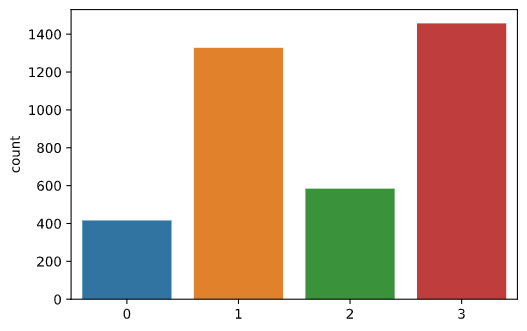
\includegraphics[scale=0.4]{img/cluster-distribution-gal.png}
\end{figure}

\begin{figure}[H]
    \centering
    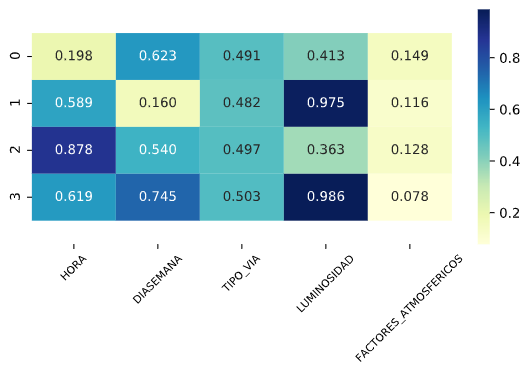
\includegraphics[scale=0.5]{img/centroides-gal.png}
\end{figure}

Podemos ver que la distribución es muy similar (aunque en este caso los grupos 1 y 3 los ha 'invertido' digamos), sin embargo, ya
se puede notar que los valores de los factores atmosféricos ha aumentado un poco, que es lo que buscábamos.

El resto de datos se puede ir viendo que tendrá una distribución muy similar, siendo los grupos 1 y 3 los accidentes producidos
de día entre lunes-miércoles y jueves-domingo, respectivamente. El tipo de vía no parece muy importante a la hora de hacer la
agrupación, al igual que los factores atmosféricos; y la luminosidad también se rige por las horas del día

Como  nos gustaría analizar todos los parámetros a la vez, al igual que antes, vamos a mostrar el grid con las gráficas de dispersión
(\textit{pairplot}):

\begin{figure}[H]
    \centering
    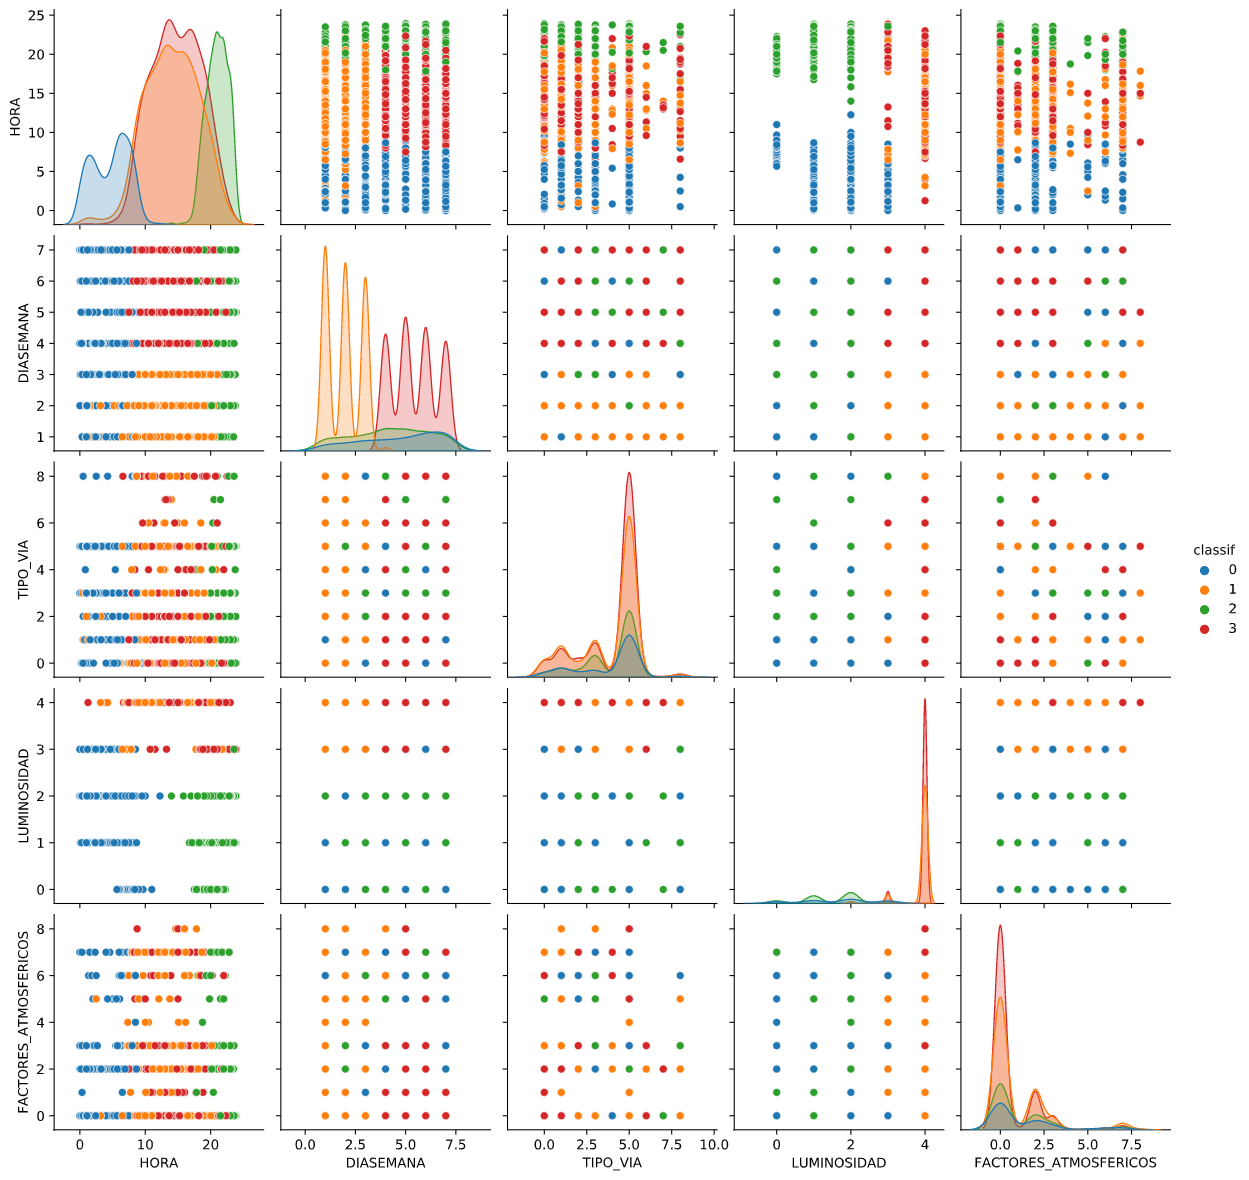
\includegraphics[scale=0.3]{img/pairplot-gal.png}
\end{figure}

Como hemos podido preveer, la distribución general es muy similar. No obstante, hay varios detalles curiosos que me gustaría comentar.
El primero de ellos es el tipo de vía, el cual parece estar mucho más distribuido que antes, para que nos entendamos, observando la
gráfica de distribución podemos notar más que antes los colores azul y verde (grupos 0 y 2); aunque siguen predominando los mismos
tipos de vías.

Pasando a los factores atmosféricos, es donde podemos observar el mayor cambio. Es cierto que la gráfica sigue teniendo un pico
importante en 'Buen tiempo', pero a diferencia de Andalucía (que no observábamos apenas datos en los otros factores atmosféricos),
en este si que hay un pico más importante sobre todo en 'Lluvia'. Esto nos quiere decir que si son un poco más comunes los accidentes
aquí por esta razón, pero por otro lado, la agrupación realizada no ha obtenido mucho cambio respecto a ello.

Por comentar algo más respecto a todo el gráfico en general, es cierto que en Galicia, tanto los accidentes por la noche, como los
accidentes con poca visibilidad, son más frecuentes que en Andalucía, ya que los colores azul y verde, que representan este grupo,
predominan más que antes.


\subsubsection*{DBSCAN}

Visto lo visto anteriormente, con lo que ha sucedido en Andalucía, nos podemos esperar lo que va a suceder con este algoritmo para
Galicia, porque como hemos analizado, las diferencias no son abismales entre uno y otro. Sin embargo, vamos a proceder de la misma
forma para comprobar si es cierto.

Seleccionamos un rango de valores tanto para epsilon como para el número de muestras, y este ha sido el resultado de la ejecución:

% Please add the following required packages to your document preamble:
% \usepackage{graphicx}
\begin{table}[H]
    \centering
    \begin{tabular}{|c|c|c|c|}
    \hline
    \textbf{epsilon} & \textbf{min\_samples} & \textbf{silhouette} & \textbf{calinsky} \\ \hline
    0.2 & 15 & -0.04054 & 127.792 \\ \hline
    0.3 & 15 & 0.24798 & 167.772 \\ \hline
    0.4 & 15 & 0.37141 & 84.054 \\ \hline
    0.2 & 20 & 0.01625 & 219.445 \\ \hline
    0.3 & 20 & 0.23841 & 181.718 \\ \hline
    0.4 & 20 & 0.37205 & 105.190 \\ \hline
    0.2 & 25 & -0.14802 & 149.848 \\ \hline
    0.3 & 25 & 0.30329 & 311.449 \\ \hline
    0.4 & 25 & 0.36697 & 131.673 \\ \hline
    \end{tabular}
\end{table}

Como era de esperar, los resultados han sido tan malos como los de Andalucía. La dinámica de crecimiento y decrecimiento de los dos
coeficientes es la misma, pero hasta con unos valores todavía más bajos. Vemos incluso que hay valores negativos en el coeficiente
de Silhouette.

Las razones de esto son las mismas que se han comentado anteriormente, y es que DBSCAN agrupa todos los datos con ruido en un cluster
aparte; y si además le sumamos que en este dataset hay menos datos, este problema se acentúa todavía más.



\newpage

% Pagina de bibliografia
\begin{thebibliography}{}
    
    \bibitem{clustering}
    Scikit-Learn. \textit{Clustering}
    \\\url{http://scikit-learn.org/stable/modules/clustering.html}

    \bibitem{pairplot}
    Seaborn. \textit{pairplot}
    \\\url{https://seaborn.pydata.org/generated/seaborn.pairplot.html}
    
    \bibitem{silhouette-score}
    Scikit-Learn. \textit{Silhouette Score}
    \\\url{https://scikit-learn.org/stable/modules/generated/sklearn.metrics.silhouette_score.html}

    \bibitem{calinsky-score}
    Scikit-Learn. \textit{Calinsky-Harabaz Score}
    \\\url{https://scikit-learn.org/stable/modules/generated/sklearn.metrics.calinski_harabasz_score.html}

    \bibitem{DBSCAN}
    Wikipedia \textit{DBSCAN}
    \\\url{https://es.wikipedia.org/wiki/DBSCAN}

    \bibitem{roc}
    Wikipedia \textit{Curva ROC}
    \\\url{https://es.wikipedia.org/wiki/Curva_ROC}
    
    \bibitem{example-pantech}
    PanTech Solutions.
    \\\url{https://www.pantechsolutions.net/road-accident-analysis-using-machine-learning}
    
    \bibitem{scaler}
    Scikit-Learn. \textit{StandardScaler}
    \\\url{https://scikit-learn.org/stable/modules/generated/sklearn.preprocessing.StandardScaler.html}

    \bibitem{clustering-seaborn}
    Seaborn. \textit{Clustering}
    \\\url{http://seaborn.pydata.org/generated/seaborn.clustermap.html}
    
    \end{thebibliography}



\end{document}